% ======================================================================
% Demo poster -- Databases and Information Systems, UHH, SuSe 2026
% A0 portrait, UHH corporate design colors. Compile with pdflatex.
% An A3 version for the moodle upload can be generated losslessly with:
%   pdfjam poster.pdf --paper a3paper --outfile poster_a3.pdf
% ======================================================================
\documentclass{article}
\usepackage[paperwidth=841mm,paperheight=1189mm,
            top=20mm,bottom=18mm,left=30mm,right=30mm]{geometry}
\usepackage{graphicx}
\usepackage{xcolor}
\usepackage{amsmath}
\usepackage[most]{tcolorbox}
\usepackage{enumitem}
\usepackage{helvet}
\renewcommand{\familydefault}{\sfdefault}
\pagestyle{empty}
\setlength{\parindent}{0pt}

% ---- UHH corporate design colors (measured from the official template)
\definecolor{uhhred}{RGB}{226,0,26}
\definecolor{uhhblue}{RGB}{0,114,182}
\definecolor{uhhgray}{RGB}{237,240,241}
\definecolor{uhhslate}{RGB}{60,81,91}

% ---- poster font sizes
\newcommand{\postertitle}[1]{{\fontsize{80}{88}\selectfont\bfseries #1\par}}
\newcommand{\postersubtitle}[1]{{\fontsize{42}{48}\selectfont\color{uhhslate}#1\par}}
\newcommand{\boxheader}[1]{{\fontsize{48}{54}\selectfont\bfseries\color{uhhred}#1\par}\vspace{6mm}}
\newcommand{\bodysize}{\fontsize{34}{43}\selectfont}
\newcommand{\smallsize}{\fontsize{28}{34}\selectfont}

% ---- gray content box in the style of the UHH info poster
\newtcolorbox{uhhbox}{
  colback=uhhgray, colframe=uhhgray, boxrule=0pt, arc=0pt,
  left=10mm, right=10mm, top=8mm, bottom=8mm,
  before skip=0mm, after skip=10mm}

\setlist[itemize]{label=\textcolor{uhhred}{\rule[1mm]{5mm}{5mm}},
                  leftmargin=14mm, itemsep=3mm, topsep=0mm}

\begin{document}\bodysize

% ================= HEADER =================
\begin{minipage}[c]{0.49\textwidth}
  
\includegraphics[width=230mm]{uhh_logo.png}
\end{minipage}\hfill
\begin{minipage}[c]{0.49\textwidth}
  \raggedleft{\fontsize{34}{42}\selectfont\color{uhhslate}
  Databases and Information Systems (DIS)\\
  Demo Presentation \textperiodcentered{} Summer Term 2026\par}
\end{minipage}

\vspace{10mm}
{\color{uhhred}\rule{\textwidth}{3.5mm}}
\vspace{12mm}

\postertitle{Demo: Forecasting a Caf\'e's Daily Ingredient Demand}
\vspace{6mm}
\postersubtitle{A Lightweight Forecasting Pipeline With Damped Triple Exponential Smoothing}
%\postersubtitle{Forecasting a caf\'e's daily ingredient demand with
%damped triple exponential smoothing}
\vspace{8mm}
{\fontsize{32}{40}\selectfont\bfseries
Bastian Queckenstedt \textperiodcentered{}
Tobias Christopher Kr\"oncke \textperiodcentered{}
Efe Enes Nayci\par}
{\fontsize{26}{34}\selectfont\color{uhhslate}
Department of Informatics, Universit\"at Hamburg\par}

\vspace{12mm}

% ================= CONTENT: two columns =================
\begin{minipage}[t]{0.54\textwidth}

\begin{uhhbox}
\boxheader{The problem}
\begin{itemize}
\item A caf\'e has records on how many cappuccinos, cocoas, espressos etc. it sold 
      in the past.
\item It must purchase the right amounts of what it will consume in the future:

\textbf{coffee beans, milk, water, cocoa, sugar, salt.}
\end{itemize}
\end{uhhbox}

\begin{uhhbox}
\boxheader{What the demo does}
\begin{itemize}
\item One year of real sales (3\,547 cups, Mar 2024 -- Mar 2025) is
      loaded \textbf{unchanged} into PostgreSQL.
\item Recipes are resolved into \textbf{six base ingredients}
      (espresso shots \textrightarrow{} 18\,g beans + 30\,ml water;
      ``milk or water'' \textrightarrow{} water).
\item A SQL \textbf{view} joins sales with recipes and aggregates the
      daily usage per ingredient -- declaratively, inside the database.
\item A Python CLI extracts one series, forecasts it, and plots the
      result automatically.
\end{itemize}
\end{uhhbox}

\begin{uhhbox}
\boxheader{Architecture}
\vspace{2mm}
\centering
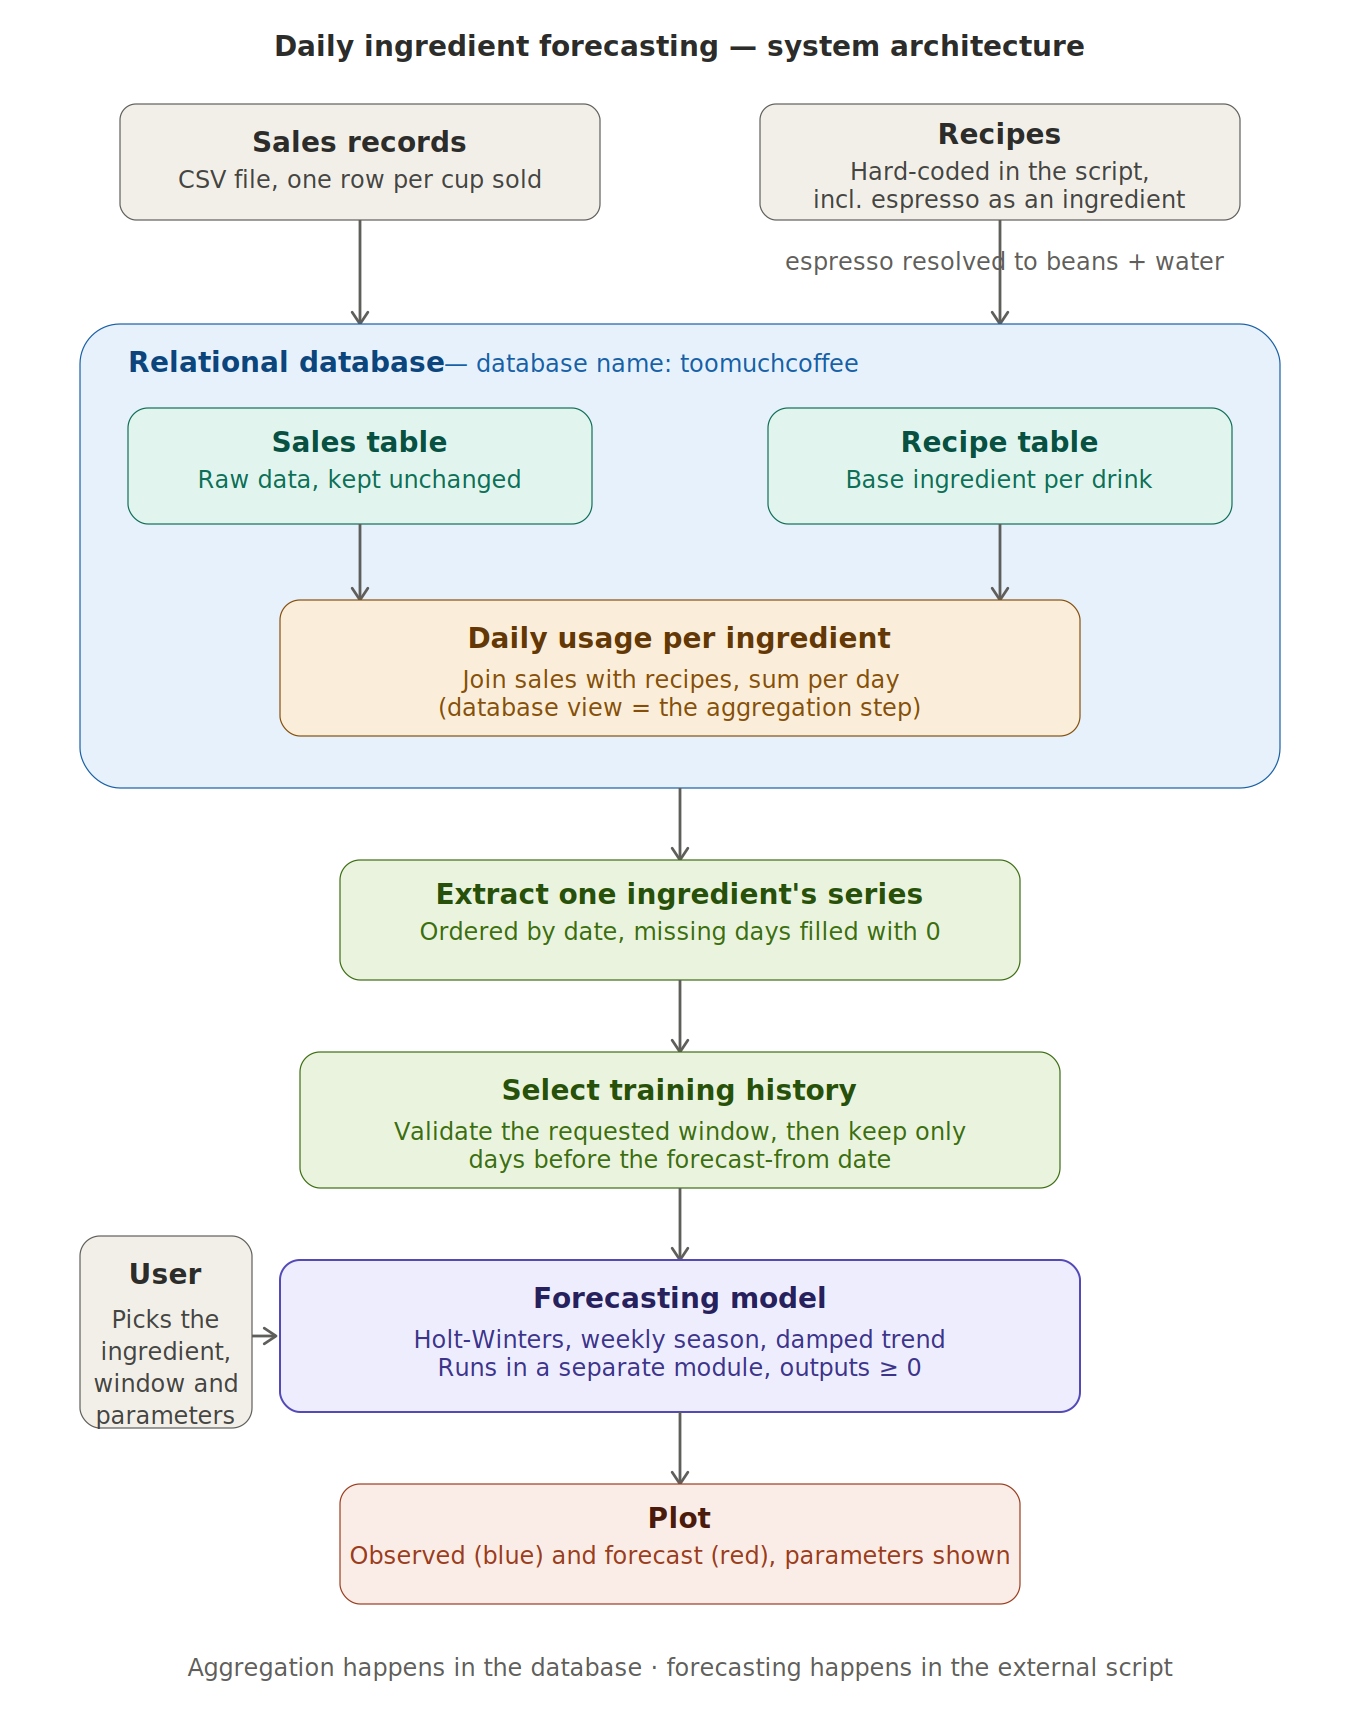
\includegraphics[width=0.78\linewidth]{dis_architecture.png}
\end{uhhbox}

%\vfill
\end{minipage}\hfill
\begin{minipage}[t]{0.45\textwidth}

\begin{uhhbox}
\boxheader{How: damped Holt--Winters}
Additive triple exponential smoothing, implemented from scratch,
season length $m=7$ days:
\begin{align*}
\ell_t &= \alpha (x_t - s_{t-m}) + (1-\alpha)(\ell_{t-1} + \phi b_{t-1})\\
b_t    &= \beta (\ell_t - \ell_{t-1}) + (1-\beta)\,\phi b_{t-1}\\
s_t    &= \gamma (x_t - \ell_t) + (1-\gamma)\,s_{t-m}
\end{align*}
\vspace{2mm}
\begin{itemize}
\item Damping $\phi<1$ lets the trend level off instead of
      exploding over long horizons.
\item Forecasts are clipped at zero -- negative usage is impossible.
\end{itemize}
\end{uhhbox}

\begin{uhhbox}
\boxheader{Try it yourself!}
Switch the ingredient, move the window, break the model:
\vspace{4mm}

{\smallsize\ttfamily
\$ timeseries.py -i milk\\
\$ timeseries.py -i "coffee beans" -a 0.3 -g 0.3\\
\$ timeseries.py -p 1.0 \quad\rmfamily\itshape (undamped trend!)\\
\ttfamily\$ timeseries.py -a 1.0 \quad\rmfamily\itshape (chasing noise!)}
\vspace{4mm}

\begin{itemize}
\item All four smoothing parameters ($\alpha,\beta,\gamma,\phi$) are
      command line flags.
\item Every run finishes in well under a second.
\end{itemize}
\end{uhhbox}

\begin{uhhbox}
\boxheader{Does it work? Validation}
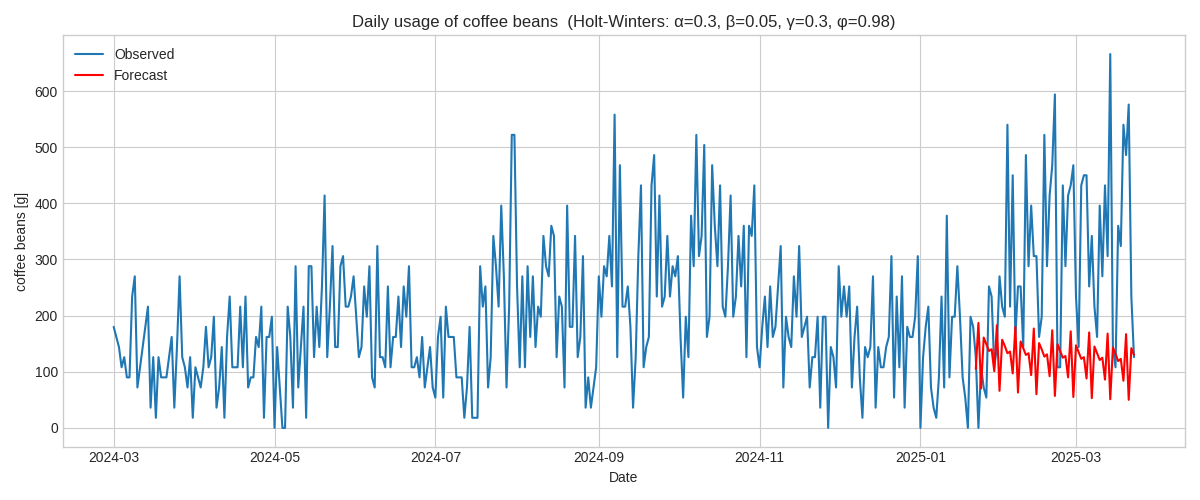
\includegraphics[width=\linewidth]{forecast_evaluation_coffee_beans_2025-01-22_2025-03-23_a03_b005_g03_p098.png}
\vspace{3mm}

{\smallsize The model forecasts the \textbf{last two observed months}
using only the history before the window -- the weekly rhythm is
clearly reproduced (coffee beans, $\alpha{=}0.3$, $\beta{=}0.05$,
$\gamma{=}0.3$, $\phi{=}0.98$).\par}
\end{uhhbox}

\begin{uhhbox}
\boxheader{Looking ahead}
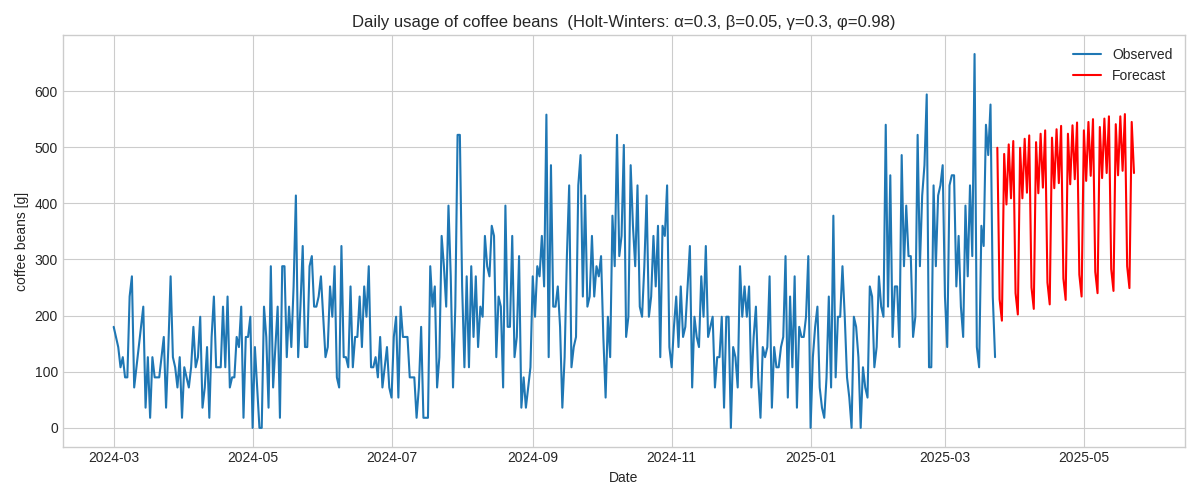
\includegraphics[width=\linewidth]{forecast_future_coffee_beans_2025-03-24_2025-05-23_a03_b005_g03_p098.png}
\vspace{3mm}

{\smallsize Two-month forecast \textbf{beyond the data}: the answer to
the caf\'e's actual planning question -- how many beans to buy next
week.\par}
\end{uhhbox}

%\begin{uhhbox}
%\boxheader{Conclusion}
%Not great, not terrible.
%\end{uhhbox}

\end{minipage}

\vfill
{\color{uhhred}\rule{\textwidth}{1.5mm}}
\vspace{4mm}

{\smallsize\color{uhhslate}
Method: Holt (1957/2004), Winters (1960), damped trend: Gardner \&
McKenzie (1985) \textperiodcentered{} Data: course datasets, DIS
SuSe 2026, Universit\"at Hamburg \textperiodcentered{} Stack: PostgreSQL,
Python (psycopg2, matplotlib), Tuxedo OS}

\end{document}
